\section{Approach} \label{sec:theory-approach}

To demonstrate the validity of the hypothesis presented above, we constructed several deep neural network models that learn to do basic arithmetic operations (namely addition, subtraction, multiplication and division) on images of handwritten digits. When properly trained, using sufficient training examples, the models can be presented with images of handwritten digits sampled from the dataset, and perform an arithmetic operation using the values depicted in the images provided.

We use the MNIST dataset to train and test our models. The MNIST dataset is a set of images depicting handwritten digits that are commonly used by image processing researchers\cite{MNIST}. Each image represents a single digit. Section \ref{sec:theory-approach-the-mnist-dataset} provides further details on the MNIST dataset. Figure \ref{fig:noisy-mnist} shows examples of the handwritten digits used from zero to nine. We refer to this type of input as noisy since there is no consistent way for rendering each digit. 

\begin{figure}[t]
	\centering
	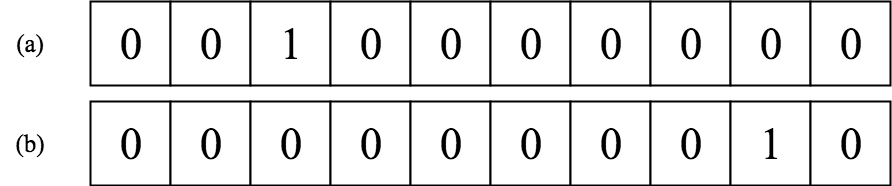
\includegraphics[max width=\textwidth]{one-hot-vector}
	\caption{Two one-hot vectors are depicted, (a) is a one-hot vector representing the integer two and (b) is another one-hot vector of the integer eight.}
	\label{fig:one-hot-vector}
\end{figure}

\begin{figure}[t]
	\centering
	
\includegraphics[max width=\textwidth]{noisy-mnist}
	\caption{Example of noisy handwritten digits sampled from the MNIST dataset.}
	\label{fig:noisy-mnist}
\end{figure}

The models are trained to output a set of one-hot vectors. One-hot vectors are vectors that have all their values set to zero except for the value corresponding to the category being represented, which is set to one. Figure \ref{fig:one-hot-vector}(a) shows an example of a one-hot vector for the number two and \ref{fig:one-hot-vector}(b) shows another example of a one-hot vector for the number eight.

Alongside the noisy handwritten digit inputs, the models are also provided a clear symbolic channel. This channel is analogous to the common language shared by human learners. The presence of symbolic inputs on this channel are controlled during training to investigate their effect on the accuracy of the network model when tested on noisy data only. Testing was performed without symbolic information to simulate the behavior of an independent agent that interacts with other agents. Our expectation is that models trained without the presence of symbols on an impoverished dataset will perform poorly on an independent test set. However, by gradually increasing the number of symbols provided during training, the model's performance should also gradually increase. Given the sequential nature of performing arithmetic operations, recurrent neural networks, like the one depicted in Figure \ref{fig:sequential-model-arithmetic}, specifically those based on long short-term memory (LSTM) units, will be used to investigate this theory. These networks will be discussed in detail in Section \ref{sec:theory-approach-methodology}.

Besides showing that the symbols help in improving the accuracy of the trained neural networks, we also want to establish an analogy between the role that symbols play in human learning and their role in improving the performance of artificial neural network models. In human learning, teachers use symbolic information in the form of examples that the learner is already familiar with to teach the learner a general method by which the learner can solve a specific problem.

Take teaching arithmetic to children for example. When teaching children how to add or divide numbers, a teacher uses objects the child is already familiar with, like apples for example, and shows the child how to relate a quantity of apples to a digit. The teacher then builds on that concept of quantity to show the learner how to add by counting one group of apples and then continue counting the other group, and how to divide by distributing the apples evenly into containers. Over time, the children gain the ability to generalize these techniques to quantities and numbers they have not encountered during learning. Symbols allow the learner to move beyond memorizing inputs and their corresponding outputs, to learn an actual algorithm that represents a general solution to the problem.

We would like to show that just as in human learning, clear symbols can expedite the learning process in artificial neural networks so as to more accurately perform arithmetic operations and provide a general solution to the problem. To show that this is possible, some of our experiments are trained on a subset of digit combinations. The independent test set is composed of combinations of digits that are not encountered during training. When the models perform well on the unseen combinations we can conclude that the artificial model has indeed learned the general arithmetic rule and is not simply doing pattern matching. 

Given the above, our goals are:
\begin{itemize}
	\item To show that it is possible to develop a deep recurrent neural network model that can learn to perform all four basic arithmetic operations (addition, subtraction, multiplication and division) more effectively with the presence of symbols than without.
	\item To explain the role that symbols play in teaching arithmetic to a machine learning system by showing that the neural network models are able to discover a principled algorithm as opposed to simply memorizing input and output patterns.
\end{itemize}

In the following sections, we describe the various network architectures and learning techniques that will be used in exploring this theory. Chapter 4 provides a detailed description of the empirical studies performed along with the results and a discussion.

\subsection{The MNIST Dataset} \label{sec:theory-approach-the-mnist-dataset}

All of our experiments use the MNIST dataset of handwritten digits. This is a database of images of handwritten digits along with labels indicating the values represented. Each digit is pre-processed so that the digit is normalized and centered in a 28x28 pixel image. The digits in the images all have the same scale and orientation. The dataset consists of 60,000 training examples and 10,000 test examples. MNIST is very popular among researchers that need to quickly test machine learning techniques since the dataset is pre-processed \cite{MNIST}. Figure \ref{fig:noisy-mnist} shows examples of MNIST digits from zero to nine.

\subsection{Multimodal Learning} \label{sec:theory-approach-multimodal-learning}

\begin{figure}[t]
	\centering
	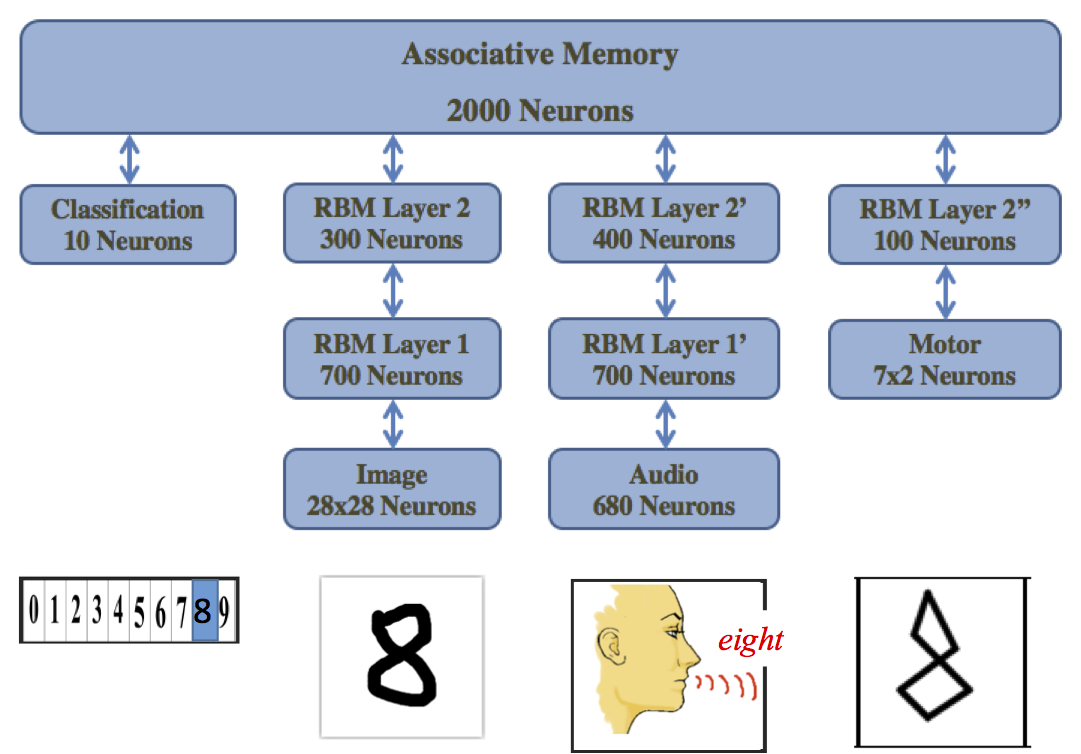
\includegraphics[max width=\textwidth]{multimodal-learning}
	\caption{A Multimodal neural network trained to communicate digits using several mediums. Each channel is modeled as a stack of Restricted Boltzman Machines connected to an associative layer\cite{iqbal2016scalable}.}
	\label{fig:multimodal-learning}
\end{figure}

Recent work by Iqbal and Silver (FLAIRS-2016 Best Paper Award)\cite{iqbal2016scalable} inspired by work by Hinton et al.\cite{Hinton:2006:FLA:1161603.1161605} and Srivastava et al.\cite{JMLR:v15:srivastava14b} has shown that it is possible to develop a multimodal deep learning system for learning a noisy handwritten digit using four sensor/motor channels (visual, audio, robotic, and symbolic) and an associative layer that ties all channels together.  After training, the presentation of a digit (sound, image, drawing) at the visible nodes of the model activates all other channels to create their associated reconstruction at their respective visible nodes. Each channel provides additional information that helps the other channels more accurately reconstruct the output. 

Figure \ref{fig:multimodal-learning} depicts the architecture that was developed as part of that work. Each channel is modeled as a stack of Restricted Boltzman Machines (RBM). A Restricted Boltzmann Machine is a generative neural network that can learn a probability distribution over its set of inputs. One important application of generative models is auto-encoding for feature engineering. Given a noisy input, an auto-encoder is able to extract a feature vector that is representative of the input based on the probability distribution being modeled\cite{pmlr-v5-salakhutdinov09a}.

\begin{figure}[t]
	\centering
	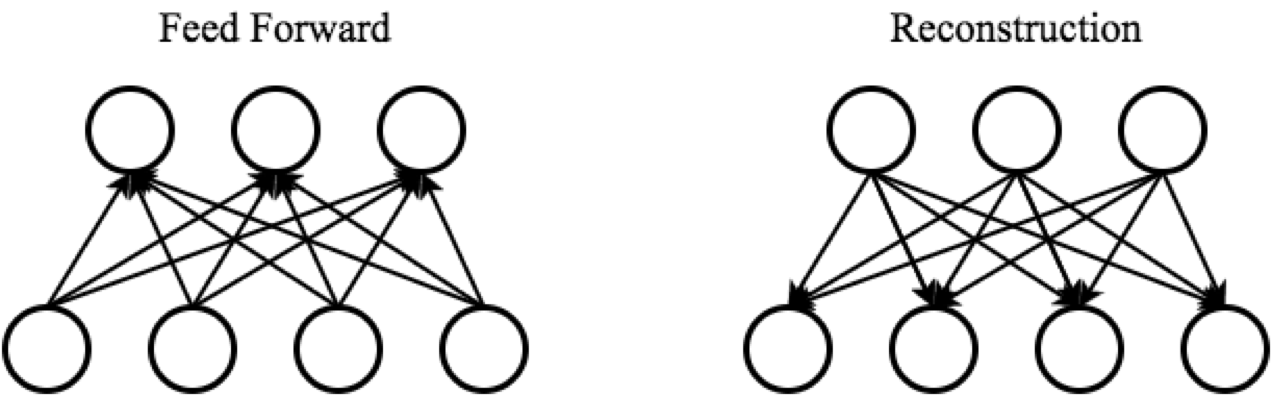
\includegraphics[max width=\textwidth]{rbm}
	\caption{An example of a Restricted Boltzman Machine showing the feed-forward pass and the reconstruction pass.}
	\label{fig:rbm}
\end{figure}

RBMs consist of an input layer and a hidden layer where the feature that represents the input is constructed. Training involves using the contrastive divergence (CD) algorithm to iteratively present the network with input examples, where an output is produced on the output layer during a feed-forward pass, and then the input is reconstructed back from that output. Figure \ref{fig:rbm} is a depiction of the architecture of an RBM showing the feed-forward and reconstruction passes. The goal of CD is to find an optimum set of weights that minimizes the reconstruction error. Contrastive divergence is an unsupervised process since there are no labels associated with the data. When fully trained, the output of RBMs is treated as a representation of the inputs that can be used in other machine learning tasks as is the case with deep belief networks\cite{Hinton:2006:FLA:1161603.1161605}.

The multimodal model developed by Iqbal and Silver\cite{iqbal2016scalable} learns to reconstruct the input presented to one channel on the other three channels each in their respective format (image, sound, robotic motion and symbol). The symbolic channel outputs the clearest signal as to which digit the multimodal deep learning system is ``thinking" about, given the input on the other channels. The symbolic channel also provides the clearest input for the other channels to generate the correct reconstructions at their visible nodes. This led us to a paper by Bengio\cite{DBLP:journals/corr/abs-1203-2990} that discusses the value of symbols and language in helping individuals learn concepts effectively without having to see all possible examples of that concept. This knowledge transfer in the form of symbols has a profound impact upon the development of our culture and the human species. 

Multimodal learning has inspired us to consider developing learning agents that learn to perform arithmetic operations using noisy channels but which can at times also receive concise information on a symbolic channel about the data on the noisy channels. The conjecture is that symbols are predominantly external communication tools that allow agents to share otherwise complex noisy concepts and in this way help them avoid local minima in model development. Clear symbols develop abstract representations that provide beneficial inductive bias during learning, therefore reducing the number of examples required to accurately learn a new concept.

\subsection{Methodology} \label{sec:theory-approach-methodology}

In this section we discuss the progression of our theory development. We provide a general overview of the neural network architectures that we are using as well as the rationale for using these architectures. There are three stages to the development of our theory. We start by describing the first stage which involves using sequential LSTM networks to perform the arithmetic operations on handwritten digits. We also discuss various techniques of supplying the symbols to our models and contrast the effectiveness of these techniques. Next, we discuss the second stage which attempts to explain the role that symbols play in improving the effectiveness of our models. Specifically, we would like to show that the networks that are trained using symbols are capable of discovering an algorithm that generalizes to all combinations of digits, instead of simply doing pattern matching, as is the goal presented above. Finally, we describe the third stage of theory development where a different representation of our symbolic channel produces the best results.

\subsubsection{Sequential Models} \label{sec:theory-approach-methodology-sequential-models}

\begin{figure}[t]
	\centering
	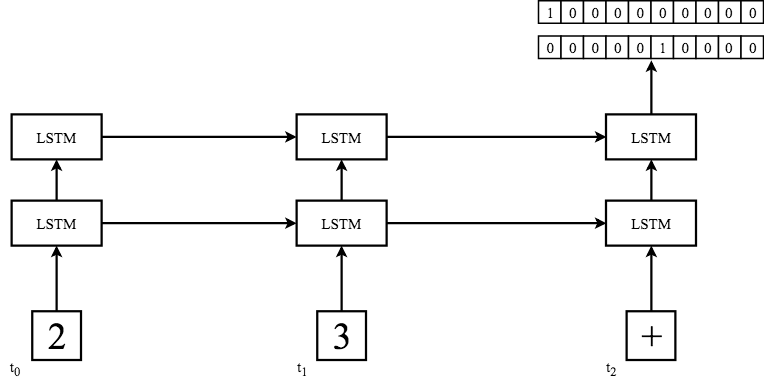
\includegraphics[max width=\textwidth]{sequential-model-arithmetic}
	\caption{A deep LSTM network that accepts a sequence of two operands and learns to perform addition on them.}
	\label{fig:sequential-model-arithmetic}
\end{figure}

When humans perform arithmetic operations, like addition, they tend to read an operand, followed by an operator, followed by another operand and then they perform the operation and produce an output. This approach to arithmetic is sequential in nature and depends on our ability to retain a representation of the operands in our minds as we read them, before we perform the operation. Given that recurrent neural networks are better suited to modeling these kinds of sequential processes, as discussed in Section \ref{sec:background-sequence-modeling}, we therefore opted to using recurrent neural networks for our experiments.

Figure \ref{fig:sequential-model-arithmetic} shows how the arithmetic expression 2 + 3 = 5 can be modeled using recurrent neural networks. On each time step the model accepts a 28x28 image of a handwritten digit from the MNIST dataset. On the last time step the model receives the operator, again in the form of a 28x28 image, and produces an output which is the result of performing the operation on the two operands. The result is represented using a pair of one-hot vectors, one vector represents the least significant digit of the result and the other represents the most significant digit of the result. Notice that we provide the operator on the final time step as opposed to the middle time step. This is because we use reverse Polish notation (RPN) when presenting the operations to the neural networks.

\paragraph{Reverse Polish Notation}

The reverse Polish notation (RPN) is a notation used to depict arithmetic expressions without the need for parentheses to indicate precedence. Unlike traditional mathematical notation where the operands of a binary operator are placed on the left and right of the operator, in RPN both operands precede the operator. The expression
\begin{gather*}
	(7 + 5) - 2
\end{gather*}
would be expressed as
\begin{gather*}
	7\ 5\ +\ 2\ -
\end{gather*}
As long as the operations have a non-variable number of operands, any arbitrarily long sequence of operations can be represented in RPN\cite{wiki:reverse-polish-notation}.

Early stack based computer models based on the work of Dijkstra and Bauer utilized RPN to reduce memory access while evaluating mathematical expressions\cite{wiki:reverse-polish-notation}. Hence, we believe that using RPN to train neural networks to perform arithmetic operations would reduce the complexity of the problem, making it easier to investigate the core hypothesis of this thesis and focus on contrasting the models' accuracy due to the presence of symbols or lack thereof instead of worrying about other factors.

\subsubsection{Symbol Channels} \label{sec:theory-approach-methodology-sequential-models}

We propose two approaches to providing the symbolic information during training. The first approach is to add an explicit input channel alongside the noisy handwritten channel. The other approach is to have the model perform a classification on each incoming noisy input, akin to the deep multi-layer models that learn to classify the MNIST dataset. By training the network to classify the input operands the architecture establishes a representation on the recurrent connections that act as an implicit symbol for each operand. When the operator is presented, it is then that the network performs the operation. The following sections provide details on these two approaches.

\paragraph{Explicit Symbols}

\begin{figure}[t]
	\centering
	
\includegraphics[max width=\textwidth]{symbols}
	\caption{Examples of the symbolic data that were used to train some of the models.}
	\label{fig:symbols}
\end{figure}

When using an explicit symbol channel, a symbol is represented as an image of the same digit presented in the noisy MNIST image,  except that they are clearly and consistently rendered in a standard font. By consistent, we mean that there are no variations between the images of a particular digit symbol. Figure \ref{fig:symbols} shows what the clear symbols look like.

\begin{figure}[t]
	\centering
	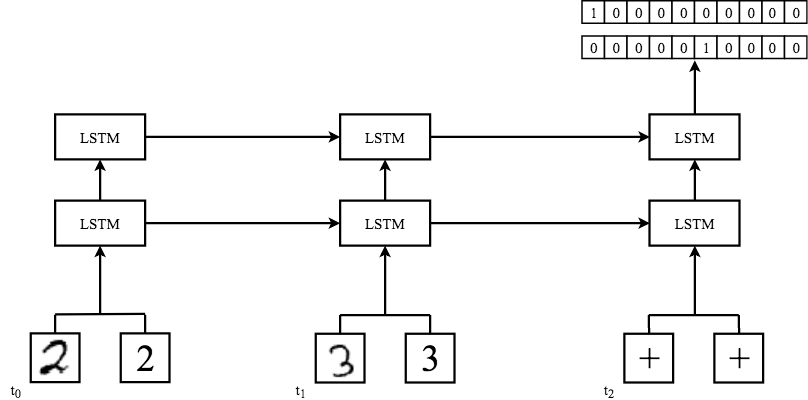
\includegraphics[max width=\textwidth]{sequential-model-with-symbols}
	\caption{A deep LSTM network that accepts a sequence of two operands and an operator each accompanied by a symbolic channel. The model learns to perform addition on the operands and produces an output in one-hot vector form.}
	\label{fig:sequential-model-with-symbols}
\end{figure}

Figure \ref{fig:sequential-model-with-symbols} shows an architecture that includes an explicit symbolic channel alongside the handwritten inputs. The network is composed of 1568 input units representing one 28x28 handwritten digit and another 28x28 image representing the clear symbol. The network outputs two one-hot vectors representing the sum of the inputs. Training is conducted by supplying sequences of three inputs; the two operands followed by the operator.

\paragraph{Implicit Symbols}

\begin{figure}[t]
	\centering
	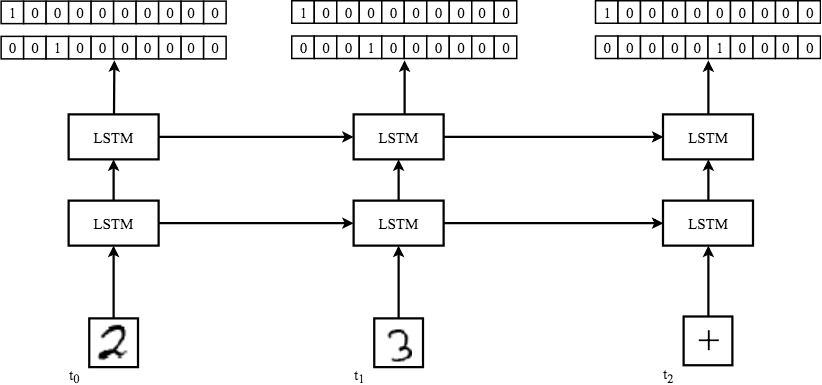
\includegraphics[max width=\textwidth]{sequential-model-with-classes}
	\caption{A deep LSTM network that accepts a sequence of two operands and an operator. The model learns to classify the operands before performing the addition when the operator is presented.}
	\label{fig:sequential-model-with-classes}
\end{figure}

Figure \ref{fig:sequential-model-with-classes} depicts an architecture that uses the second approach of implicit symbols. Here the network does not include a symbolic channel with the inputs. Instead, the network accepts 784 input units representing a 28x28 handwritten digit, one at a time. Each time a handwritten digit is provided, the model is trained to produce the value of that digit on the output channel. If an arithmetic operator is provided to the network, the model will output the result of the operation on the previous inputs. We believe that teaching the network to properly classify the inputs before performing the operation is similar to training the model using the clear symbolic inputs. The LSTM layers should be able to maintain the classes learned within their context, therefore, providing the same utility a symbolic channel would provide.

\bigskip

Symbols provide consistency that the neural network models can use to learn to perform the mathematical operations instead of relying solely on the noisy handwritten inputs. By successfully mapping the noisy inputs to the clear symbols, the job of the learning system becomes discovering a set of rules that accepts the clear symbols along with an operator to produce a result. Without the presence of these symbols, our neural networks would be susceptible to the high variation exhibited by the noisy inputs and therefore would need more training examples, making learning expensive.

We can explain the role of the symbol channel in terms of Bayesian inference. The probability of finding an optimum representation $h$ in the hypothesis space is affected by the presence of evidence, in our case, the classification data $C$ (symbols) and the noisy training data $D$. From Bayes' Theorem this can be given as:
\begin{equation}
p(h|C,D) = \frac{p(C,D|h) \cdot p(h)}{p(C,D)}
\end{equation}
The Maximum a posteriori hypothesis (assume prior hypotheses are equally likely, and data is common divisor) is given by:
\begin{equation}
h_{MAP} = \argmax_h p(C,D|h) p(h)
\end{equation}
However, $p(C,D|h) \cdot p(h)$ can be expressed as:
\begin{equation}
\begin{split}
p(C,D|h) \cdot p(h)\\
& = \frac{p(C,D,h)}{p(h)} \cdot p(h)\\
& = p(D | C, h) \cdot \frac{p(C, h)}{p(h)} \cdot p(h)\\
& = p(D | C, h) \cdot p(C |h) \cdot \frac{p(h)}{p(h)} \cdot p(h)\\
& = p(D | C, h) \cdot p(C |h) \cdot p(h)
\end{split}
\end{equation}
This means that the best hypothesis is the one that maximizes the product of the probability of the hypothesis, $p(h)$, the probability of the correct symbol given a hypothesis, $p(C |h)$, and the probability of the correct arithmetic operation given both the correct symbol and the hypothesis, $p(D | C, h)$\cite{wiki:Bayesian_inference}. Therefore, correctly mapping the noisy digits to the classes increases the likelihood that the learning system will discover a hypothesis that will maximize the posteriori probability. The next section further develops our approach by explaining empirical techniques that we can use to better understand the role of symbols.   

\subsubsection{Pattern Matching Verses Learning an Algorithm} \label{sec:theory-approach-methodology-pattern-matching-vs-learning-an-algorithm}

In the introduction to Section \ref{sec:theory-approach} we laid out our objectives from this research, namely to show that it is possible to improve the effectiveness of deep neural network models using symbols when training using an impoverished dataset and to also show that the presence of symbols allows the model to discover a general solution to the problem similar to how symbols affect the ability of humans to learn. In the previous two sections, we described the first stage of our theory development that aims to satisfy the first objective. Here we further develop our theory and attempt to satisfy the second objective by showing that without symbols the ability of neural networks to find a general solution to the problem is diminished.

\paragraph{Pattern Matching}

We explained in Section \ref{sec:theory-hypothesis} the concept of multi-task learning and described how the common representation shared by both the symbolic inputs and the noisy handwritten digits can make learning more effective. Learning from the noisy handwritten digits alone is difficult due to the high number of variations presented to the model. The presence of clear symbols guides the neural network to discover a good representation in its hidden weights, that can be used to identify the various noisy handwritten digits. The model then learns to perform a mapping or pattern matching between the digits and the desired outcome of the arithmetic operation.

\begin{figure}[t]
	\centering
	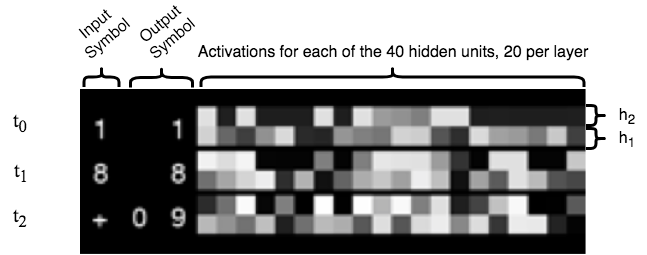
\includegraphics[max width=\textwidth]{activations-cluster}
	\caption{A visualization of hidden layer activations of a deep recurrent network with three time steps and two hidden layers 20 units each. The activations are the result of presenting the model with the operation: 1 + 8, in reverse Polish notation}
	\label{fig:activations-cluster}
\end{figure} 

To verify that this is indeed what is happening, we need to understand the relationship between the network's inputs and the state of its hidden layers. We therefore use a visualization technique, known as activations clustering, that captures the value of $h_t$ on each hidden layer and renders these as intensities in an image. The output value of each unit in the hidden recurrent layers is mapped to a pixel intensity where an output of -1 would map to 0 and an output of 1 would map to 255. Each unit would be assigned a region on the activations cluster. Figure \ref{fig:activations-cluster} shows an activations cluster for a recurrent network with three time steps and two hidden layers, 20 units each. Our expectation is that the clusters obtained from the model trained using symbols would show the consistency described above. This means that when the same combination of digits and operation is presented to the network, regardless of the instances of the MNIST digits used, a particular region of the cluster would show the same pattern. We also expect that when we contrast this behavior with that of a model trained without the presence of symbols, no such pattern would be apparent.

Besides observing this consistency in the hidden layer activations, we would expect to see some patterns emerge as well. For example, the ``carry one" concept that humans use to do complex addition and that forms an important function in binary arithmetic, might be represented in the network's hidden layers. Since discovering such patterns would be easier with clear symbols than with noisy handwritten digits, the presence of symbols should significantly improve the ability of the neural networks to achieve this goal. Consider the operations 8 + 1 and 8 + 2. The first does not produce a carry whereas the second does. We expect that by examining activations clusters produced for these two operations, we would observe a transition in some part of the network that indicates a carry being generated. Discovering this carry concept is a major step towards developing a learning system that is able to generalize in the same way humans can.

\paragraph{Learning an Algorithm}

To satisfy our second object, we would like to show that symbols help the learning process advance beyond the ability to do pattern matching effectively and instead actually learn the general algorithm that performs the arithmetic operation. Showing that this is the case would support the use of symbols in neural network learning analogous to their use in human learning, for example when children learn arithmetic as described in Section \ref{sec:theory-approach}. Our approach involves developing recurrent neural networks that are trained on only a subset of the dataset and then tested on the remaining examples in the dataset. We believe that without the presence of symbols it would be very difficult for an artificial neural network to perform well, just like human learners that learn without the knowledge shared by other agents. By providing symbols during training, our models should be able to generalize to the unseen examples and therefore show that an algorithm has been developed.


\subsubsection{Temperature Encoding} \label{sec:theory-approach-methodology-temperature-encoding}

\begin{figure}[t]
	\centering
	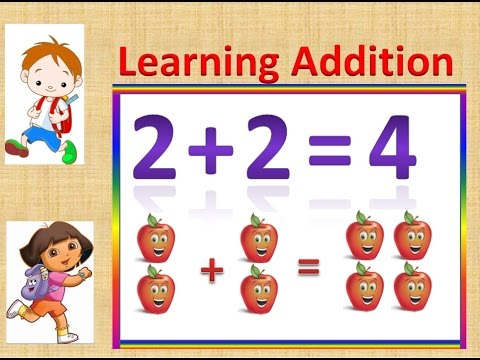
\includegraphics[max width=0.5\textwidth]{children-addition}
	\caption{An image that uses pictograms of apples to teach small children how to perform addition. Here children are taught to add 2 + 2 by counting two apples and then counting another two apples to make four apples\cite{learning_2015}.}
	\label{fig:children-addition}
\end{figure}

In the previous section, we discussed two methods by which symbols can guide our neural networks to develop good representations. We believe a neural network model can discover functions such as carry forward, especially if a clear symbol is present that allows the model to learn a consistent representation of the input handwritten digits. However, discovering an algorithm that generalizes to unseen digits is not straightforward since the model will not have learned this unseen sequence of digits before. In this section we describe the third and final stage of our theory development that we believe will overcome this difficulty.

In the beginning of this chapter we gave an example of how children learn to perform arithmetic using familiar objects. Figure \ref{fig:children-addition} depicts how this process works. Learners are presented a problem of adding 2 + 2 to produce 4. The problem is presented using traditional mathematical symbols such as the digits and the plus operator. Below the digits, pictures of apples are also used to convey the meaning of the digits and mathematical operator. Children are taught that performing the 2 + 2 operation is like counting two apples and then counting another two apples to obtain four apples.

Over time, human learners gain the ability to map the images of these familiar objects to the digits, especially to the quantities represented by the digits, and that performing arithmetic operations on the digits depends on the ability of the learner to successfully make this mapping. Children then later develop the ability to translate digits into quantities without the need for symbols of the digits. They are also able to perform these arithmetic operations without having to memorize every possible combination of digits, instead relying on the general solution they acquired with the aid of this symbolic knowledge.

In order to establish the analogy between learning with symbols in humans and learning with symbols in artificial neural networks we must show that we can develop a learning system that is able to learn:
\begin{itemize}
	\item the ordinal relationships between the digit operands, also known as successorship,
	\item the quantity or size each digit represents, and
	\item the function of the operator.
\end{itemize}
Human learners are able to use the knowledge transferred through the use of the symbols described above to capture all three aspects. The clear symbols provided to our neural network models should in turn be able to also represent these aspects\cite{wiki:Elementary_arithmetic}. 

When contrasting the symbols used by children to learn arithmetic and our proposed symbols, we notice that our one-hot vector representation lacks the ability to convey these aspects. The apples in Figure \ref{fig:children-addition} for example clearly indicate to a child the quantity represented by the digits. It also allows the learner to compare quantities and determine an ordinal relationship between the quantities and their respective digits. The one-hot vector symbols however do not have that ability.

\begin{figure}[t]
	\centering
	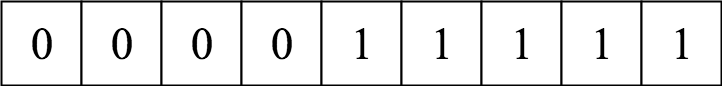
\includegraphics[max width=\textwidth]{temperature-encoding}
	\caption{The number 5 encoded in a vector using temperature encoding.}
	\label{fig:temperature-encoding}
\end{figure}

To overcome this problem, we need a better representation for our symbols. We therefore propose encoding the symbols using temperature encoding. A temperature encoded integer is a vector of binary values that has as many values sequentially set to one, starting from the right, as the integer being represented. Figure \ref{fig:temperature-encoding} is a depiction of the digit 5 encoded using temperature encoding. This type of encoding was chosen because, besides providing a clear vector representation for the digit, it also conveys the quantity of the digit that allows the model to capture the ordinal relationship between the digits. We expect that this will work better than one-hot encoding for learning an algorithm that can generalize to previously unseen digit combinations.
